\begin{figure}[htbp]
  \begin{tabular}{cc}
    \begin{minipage}{0.5\hsize}
      \includegraphics[width=5cm]{../pic/Dron/K0_peak_wBG.eps}
    \end{minipage}
    \begin{minipage}{0.5\hsize}
      \includegraphics[width=5cm]{../pic/Dron/K0_peak.eps}
    \end{minipage}
  \end{tabular}
  \caption{
    These figures show the $K^0 \rightarrow \pi^+ \pi^-$ decay peak in $K^- d \rightarrow n \pi^+ \pi^ n$ events.
    The left figure displays the $K^- d \rightarrow n \pi^+ \pi^- n$ event spectrum (black line)
    along with the MC simulated background (gray line).
    The right figure presents the background-subtracted spectra and the fit results.
  }
  \label{fig:reso:K0_peak}
\end{figure}

\begin{figure}[htbp]
  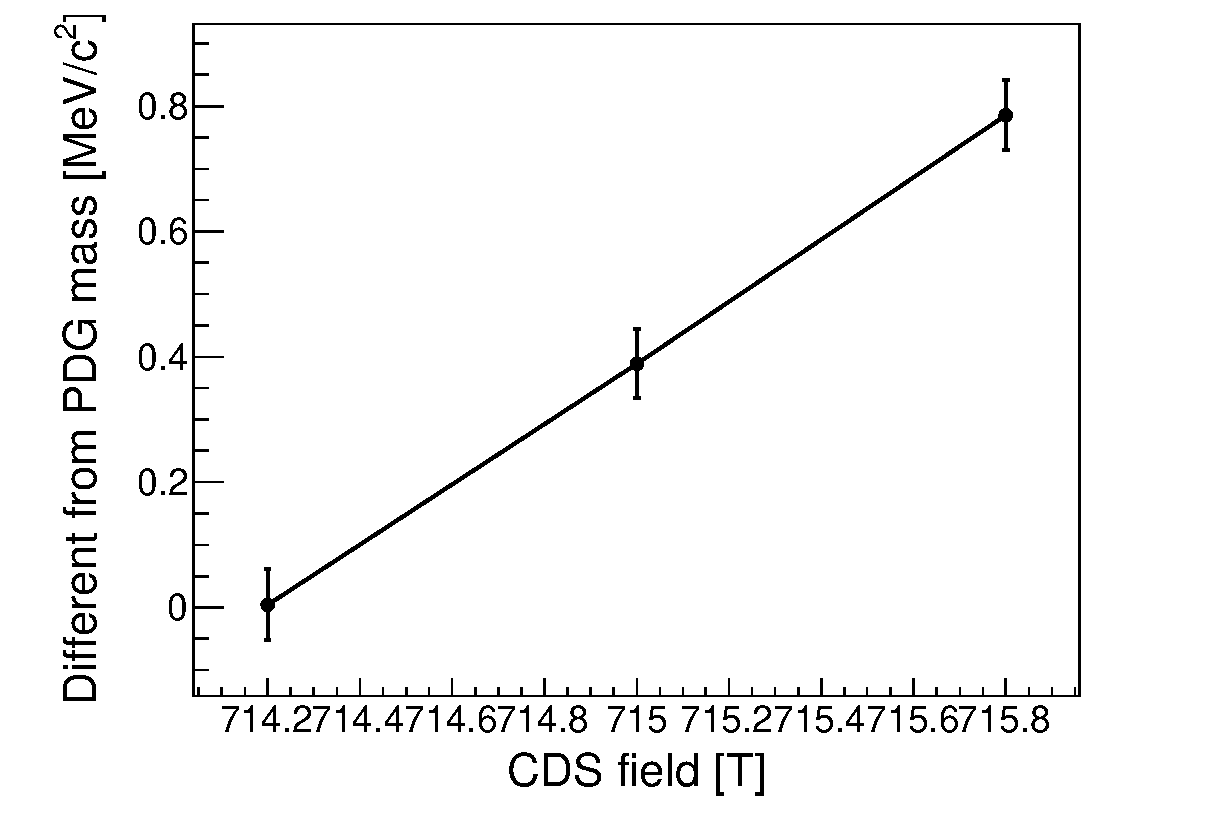
\includegraphics[width=5cm]{../pic/Dron/CDC_field.eps}
  \caption{
    This figure shows the relationship between the magnetic field settings of the CDC in the analysis and the center value of the $K^0$ peak.
  }
  \label{fig:reso:CDC_field}
\end{figure}


As explained in Section \ref{sec:???}, the CDS measures the momentum of charged particles by tracking their trajectories in a magnetic field.
The resolution of the CDS is estimated using events
in which the $K^0$ produced in the $K^-d \rightarrow n n K^0$ reaction decays into $\pi^+$ and $\pi^-$.
This reaction is one of the $K^-d \rightarrow n \pi^+ \pi^- n$ final states described in Section \ref{sec:npipin_decompose},
and this final state is fully reconstructed as explained in Section \ref{sec:template_fitting}.
Therefore, by subtracting reactions other than $K^0$ production, only the peak can be extracted, as shown in Figure. \ref{fig:reso:K0_peak}
The magnetic field of the CDS is measured using a Hall probe, and fine-tuning is performed based on the $K^0$ peak.
As shown in the Figure \ref{fig:reso:CDC_field},
this was done using selected values of the CDS magnetic field applied in the experimental data analysis.
The field was slightly adjusted from the default value of ???T and was finally determined to be ???T.

The momentum resolution is based on the positional resolution of the CDC.
To determine the positional resolution that best reproduces the width of the observed $K^0$ peak,
the correlation between the positional resolution of the CDC and the width of the $K^0$ peak in the MC simulation was examined,
as shown in Figure \ref{fig:???}.
From this, the positional resolution was estimated to be 200$\mu m$.
